
\chapter{用户画像模块}
\section{引言}

小米手机主题用户画像是根据用户社会属性、生活习惯和消费行为等信息而抽象出的一个标签化的用户模型。构建用户画像的核心工作包括:1、给用户贴标签,而标签是通过对用户信息分析而来的高度精炼的特征标识。2、对每个用户标签赋予一定权重以代表该用户对该标签的偏好度。\autoref{pic:hl_userProfile}所示为一个典型的用户画像,标签面积越大代表其权重越高。小米手机主题用户画像的标签是结构化的,最下层是用户基础信息,包括姓名、年龄、经纬度、职业等,中层是用户的兴趣标签,如正太控、动漫控、运动达人等,最上层是抽象标签,如高、中、低忠诚度用户,高、中、低价值用户等,所以对于用户画像的建模过程,就是不断的丰富标签和抽象标签的过程。具体工作包括:从各个维度上对人群细分,完善画像体系,同时针对每类细分人群,丰富群体特征。


\section{用户画像数据类型}
在个性化服务的用户画像建模中,一个完整、成熟的用户画像是包含基础静态数据类型、基础行为数据类型和高维数据类型。
\subsection{基础静态数据类型}
当一个新用户注册时会填写人口基本信息,通过json格式从客户端传回服务器,格式\autoref{code:registe}
\begin{lstlisting}[language=json,firstnumber=1,label={code:registe}]
    {"registerLog": {
      "userId": "001",
      "gender": "male",
      "profession": "student",
      "phone": "null",
      "borthday": "19860820",
      "isWeiboUser": "no",
      "isWeixinUser": "yes",
      "city": "北京市",
      "timestamp": "1453700393",
      "...": "..."
    }}
\end{lstlisting}

\label{chap:example}
\begin{figure}
\centering
  \framebox{\includegraphics[scale=0.35]{figures/hl_userProfile}}
  \figcaption{用户画像标签示例图}
  \label{pic:hl_userProfile}
\end{figure}
有的用户会利用微信、微博提供的第三方免登陆API,第三方数据可以用来交叉验证用户填写的基础信息数据。用户每次登陆时应用程序还会获得其手机品牌、操作系统等信息。因此,通过解析server log得到基础静态数据形式:
  \begin{table}[htp]
  \centering
  \tabcaption{用户-基础静态数据矩阵表}
  \label{tab:tagweight}
  \begin{tabular}{|c|c|c|c|c|c|c|c|} \hline
   用户id & 性别 & 年龄 & 职业 & 电话号码 & 手机运营商 & 是否为微博用户 & ... \\ \hline
   001 & 女 & 23 & 学生 & 13948572214 & 移动 & 是 & ... \\ \hline
   002 & 男 & 30 & 学生 & 15811036703 & 移动 & 是 & ... \\ \hline
   ... & ... & ... & ... & ... & ... & ... & ... \\ \hline
  \end{tabular}
  \end{table}

  \subsection{基础行为数据类型}
  基础行为数据是指用户的一些行为,包括购买,试用,浏览,评价等的统计量,用户行为数据格式如\autoref{code:registe}
    \begin{lstlisting}[language=json,firstnumber=1,label={code:registe}]
      {"actionLog": {
        "userId": "001"
        "actions": [{
            {"itermId": "0822"},
            {"actionType": "jumpIn"},
            {"stayTime": "32000"},
            {"clickNum": "2"},
            {"scrollNum": "5"},
            {"timestamp": "1453701393"},
            {"...": "..."}
        }]
      }}
    \end{lstlisting}
  基础行为数据作为用户行为统计量可以反映用户的活跃度、消费能力和用户类型,基础行为数据形式如\autoref{tab:taglower}。
    \begin{table}[htp]
    \centering
    \tabcaption{用户-基础行为数据表}
    \label{tab:taglower}
    \begin{tabular}{|c|c|c|c|c|c|c|c|} \hline
     用户id & 购买 & 试用数 & 浏览 & 未支付订单数 & 活跃时间段 & 日浏览时长 & ... \\ \hline
     001 & 2 & 7 & 118 & 0 & 20:00-22:00 & 120 & ... \\ \hline
     002 & 0 & 3 & 7 & 1 & 13:00-14:00 & 60 & ... \\ \hline
     ... & ... & ... & ... & ... & ... & ... & ... \\ \hline
    \end{tabular}
    \end{table}

  \subsection{高维数据类型}
  高维数据即用户的抽象标签,是用户画像模型从基础静态数据和基础行为数据统计、分析、抽象出来,用来衡量用户某一方面的价值,如用户信用是指是否有过作弊行为、退款次数过多等综合评估,用户价值是指购买次数、单笔消费额、消费频率的综合评估,高维数据形式如\autoref{tab:taghigh}。
    \begin{table}[htp]
    \centering
    \tabcaption{用户-高维数据表}
    \label{tab:taghigh}
    \begin{tabular}{|c|c|c|c|c|c|c|c|} \hline
     用户id & 信用 & 价值 & 忠诚度 & 活跃度 & 价格敏感度 & 奖励敏感度 & ... \\ \hline
     001 & 高 & 高 & 高 & 高 & 低 & 低 & ... \\ \hline
     002 & 中 & 中 & 高 & 高 & 高 & 高 & ... \\ \hline
     ... & ... & ... & ... & ... & ... & ... & ... \\ \hline
    \end{tabular}
    \end{table}

  \section{用户画像建模}
  用户画像建模的过程就是原始数据进过处理、分析得到可信度高的用户标签信息的过程,对于不同类型的用户数据其建模的侧重功能点也有所区别。
  \subsection{基础静态数据建模}
  用户基础静态数据的特点是数量不多,但在推荐系统中所占的权重较大,因此对其可信度要求较高,在对基础静态数据建模的时候主要实现俩个功能:根据上下文信息补全为空的标签和根据上下文信息校验已有的标签。

  标签补全以用户性别标签为例,新用户注册时如未填写性别信息其值会默认设为Null,方便用户画像建模时判断。主要思路是通过分析用户上下文信息,包括第三方登入数据、用户语音和头像获得用户真实的性别,如以上方法都未成功获取用户性别,程序会利用线性回归算法挖掘出一个最有可能的性别标签值,代码:
  \begin{lstlisting}
    public String getUserGender(String log) {
        Gson gson = new Gson();
        UserProfile userProfile = gson.fromJson(log, UserProfile.class);

        if (userProfile.gender != null) {
            return userProfile.gender;
        }

        String useId = userProfile.useId;
        //通过第三方应用登陆数据得到用户信息
        UserProfile thirdPartUP = gson.fromJson(getThirdPartUserInfo(useId), UserProfile.class);
        if (thirdPartUP.gender != null) {
            return thirdPartUP.gender;
        }

        //通过分析用户语音数据得到用户信息
        UserProfile voiceUP = gson.fromJson(getUserVoiceUserInfo(useId), UserProfile.class);
        if (voiceUP.gender != null) {
            return voiceUP.gender;
        }

        //通过线性回归算法挖掘出用户信息
        UserProfile lrUP = gson.fromJson(getLinearRegressionUserInfo(useId), UserProfile.class);
        return lrUP.gender;

    }
  \end{lstlisting}

  标签校验是指虽然相关信息已经被填写,但程序认为其值具有随意性,需要根据上下文信息加以确认并校验,标签校验由于考虑的因素较多导致计算量大,使得其应用场景较少,还是以用户性别标签为例,代码如\autoref{code:check_tag}
  \begin{lstlisting}[language=java,firstnumber=1,label={code:check_tag}]
      public String getRightUserGender(String log) {
      int[] count = {0, 0};
      Gson gson = new Gson();
      UserProfile userProfile = gson.fromJson(log, UserProfile.class);

      if (userProfile.gender != null) {
          if (userProfile.gender.equals("male")) {
              count[0]++;
          } else {
              count[1]++;
          }
      }

      String useId = userProfile.useId;
      UserProfile thirdPartUP = gson.fromJson(getThirdPartUserInfo(useId), UserProfile.class);
      if (thirdPartUP.gender != null) {
          if (thirdPartUP.gender.equals("male")) {
              count[0]++;
          } else {
              count[1]++;
          }
      }

      UserProfile voiceUP = gson.fromJson(getUserVoiceUserInfo(useId), UserProfile.class);
      if (voiceUP.gender != null) {
          if (voiceUP.gender.equals("male")) {
              count[0]++;
          } else {
              count[1]++;
          }
      }

      UserProfile lrUP = gson.fromJson(getLinearRegressionUserInfo(useId), UserProfile.class);
      if (lrUP.gender.equals("male")) {
          count[0]++;
      } else {
          count[1]++;
      }
      if (count[0] >= count[1]) {
          return "male";
      } else {
          return "female";
      }
  }
  \end{lstlisting}

  \subsection{基础行为数据建模}
  基础行为数据建模更新频率较快,计算量较大,因此采用离线方式利用sql语句从hive表中得出用户在一段时间区间内特定行为的统计数据。需要注意一些用户行为的延迟性,如购买行为,从下单到支付成功可能跨越若干天,因此约定订单量以支付时间为准,有时候遇到网络故障相同订单会被用户提交多次,需要利用distinct做去重操作。统计特定用户某段时间的订单量的sql语句如\autoref{code:order_sql}
  \begin{lstlisting}[language=SQL,firstnumber=1,label={code:order_sql}]
    set hiveconf:ymdwithline=2016-04-06;
    set hiveconf:userId=525108009;

    select count(distinct a.order_id) score
    from theme_dw.dw_v_order_base
    where concat_ws('-',year,month,day) between date_sub('${hiveconf:ymdwithline}',5) and '${hiveconf:ymdwithline}'
    and userId='${hiveconf:userId}'
    and finish_time like '${hiveconf:ymdwithline}%'
  \end{lstlisting}

  \subsection{高维数据建模}
  高维数据建模的数据来源包括基础静态数据、基础行为数据,数据类型包括累计量和趋势量,累计量包括用户浏览总数、用户购买总数等,趋势量是指用户最近登录时间、最近购买时间等,利用数据挖掘分类算法得出一个训练模型,需要注意的是用户行为类型、发生时间、发生位置会影响模型的权重计算,即weight = (行为类型 + 时间上下文 + 空间上下文) × 时间衰减因子。其中,用户行为类型包括浏览、购买、搜索、评论、购买、点击赞、收藏等,我们定义购买权重计为5,而浏览仅仅为1。空间上下文是指用户跳转入口方式,我们定义搜索入口权重3,排行榜入口为2。时间上下文是指用户之前是否接触过此类标签,接触频率等。时间衰减因子根据半衰期公式得出,如所示\autoref{equ-half_life},其中T取值为1,t为行为发生时间距离当前时间的天数。
  \begin{equation}
    score=(\frac{1}{2})^{(t/T)}
    \label{equ-half_life}
  \end{equation}

  以用户活跃度为例,由于日活跃变动过大,月活跃过于滞后,因此按周统计,模型选择线性回归算法,模型输入为基础静态数据、基础行为数据,模型输出为一个int型整数,值为[1,2,3],分别对应不活跃、较活跃、活跃。代码,代码如\autoref{code:check_user_active}
  \begin{lstlisting}[language=java,firstnumber=1,label={code:check_user_active}]
    public int getActivityScore(String userId) throws Exception {
        String userBaseInfo = getUserBaseInfo(userId);
        String userActionLog = getUserActionLog(userId);
        Gson gson = new Gson();
        String score = getLinearRegressionActivityScore(
          gson.fromJson(userBaseInfo, UserProfile.class), 
          gson.fromJson(userActionLog, UserActions.class));
        double activityScore = Double.parseDouble(score);
        if (activityScore >= 66) {
            return 3;
        } else if (activityScore >= 33) {
            return 2;
        } else {
            return 1;
        }
    }
  \end{lstlisting}

  \section{实验与分析}
  本节的研究目标是如何利用用户画像给新注册用户做出准确的Top-N推荐并提升用户留存率。严谨的AB测试流程应该先分析AA测试,得出实验本身自带的误差,然后利用这个误差因子修正AB测试结果,最终得到统计结果,但AA测试会严重拖慢节奏,所以本节只重点介绍AB测试。实验最终用户人群为北京地区,所有从2015年9月1号到2015年9月7号这段时间注册的用户,去除用户注册信息不完整后用户数为20万,对照组和测试组a和测试组b人群比例为33.3:33.3:33.4,对照组用户人群的推荐结果没有利用用户画像,测试组a人群的推荐结果只包含热门主题,测试组b人群的推荐结果利用了用户画像,对照组和测试组b的推荐候选集为全部主题,测试组a的推荐候选集为Top 20\%热度的主题。。实验从2015年9月8号开始到2015年10月8号结束,周期为一个月。用户画像建模如\autoref{code:create_table}。
    \begin{lstlisting}[language=json,firstnumber=1,label={code:create_table}]
      {
      //静态数据
      user_id                  int    comment '用户id',
      user_name                int    comment '用户name',
      user_age                 int    comment '用户age',
      create_time              string comment '账号创建时间',
      city_id                  int    comment '城市id',
      city_name                string comment '城市名',
      phone                    int     comment '手机号',
      os_version               stringt comment '操作系统及版本',
      phonetype_serial         string  comment '手机品牌及型号',
      education_level          string  comment '学历',
      school                   string  comment '学校',

      //行为数据
      click_num int comment '点击次数',
      last_click_time int comment '最近点击时间',
      buy_num int     comment '购买次数',
      last_buy_time int     comment '最近购买时间',
      try_use int     comment '试用次数',
      last_tryuse_time int     comment '最近试用时间',
      browse_num int     comment '浏览次数',
      last_browse_time int     comment '最近浏览时间',
      browse_total_time int     comment '浏览总时长',
      login_num int     comment '登陆总次数',
      login_total_time int     comment '登陆总时长',
      comment_num int     comment '评论总次数',

      //高维数据
      use_time                 int     comment '使用时间段',
      not_use_time             int     comment '沉默天数',
      friendship               list<bigint>  comment '好友关系',
      friend_group             list<bigint>  comment '好友圈',
      coupon_sensitivity_score decimal(20,4) comment '券敏感及阈值',
      purchase_will_score      decimal(20,4) comment '消费意愿',
      loyal_score              decimal(20,4) comment '忠诚度',
      credit_score             decimal(20,4) comment '活跃度'
      }
    \end{lstlisting}
    \subsection{评测指标}
    本节使用线上A/B测试方案\citep{ab-test},利用用户留存率来评测推荐系统应对冷启动问题的效果。用户留存数是指在某段时间开始使用App应用,经过一段单位时间后仍然继续使用该App应用的用户,用户留存率是指用户留存数占当时新增用户的比例,计算单位取天,用户留存率研究对象为新注册用户,反映了推荐系统的转换能力,即由初期的不稳定的用户转化为活跃、稳定、忠诚的用户。
    \subsection{对比模型}
    \autoref{pic:hl_saveRatio}展示了不同模型的实验结果。我们对比了单纯的推荐模型、推荐热门商品的简单推荐模型和融合了用户画像的推荐模型在新注册用户数据集上的用户留存率。图中,横坐标是时间变量,单位为天,纵坐标是用户留存率,每一条曲线代表了一个模型的用户留存率随时间变化的曲线。通过观察曲线可以发现用户留存率随时间流动呈指数分布,头三天就流失了约90\%的新用户,从第四天用户留存率开始停留在一个比较稳定的阈值,为减少误差头三天的数据不记入统计数据,统计结果显示,融合了用户画像的推荐模型的留存率是10.3\%,比推荐热门商品的简单推荐模型的留存率8.19\%高了2.11个百分点,相对于单纯的推荐模型的留存率5.76\%高了4.54个百分点。由此可见用户画像能够很好的解决冷启动问题并得到较高的新注册用户留存率。
    \begin{figure}
    \centering
      \framebox{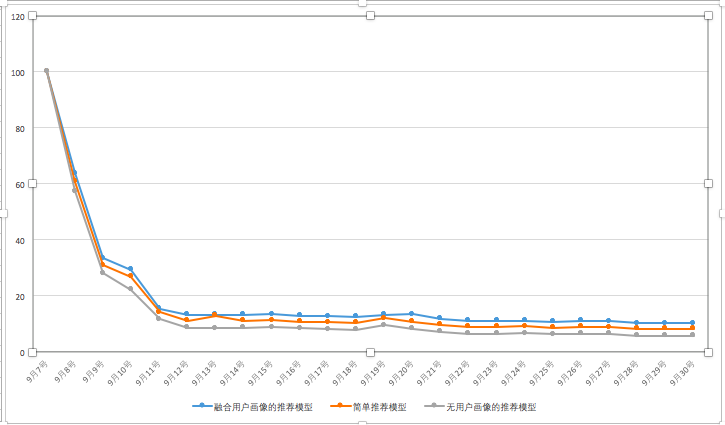
\includegraphics[scale=0.55]{figures/hl_saveRatio}}
      \figcaption{新用户留存率实验对比图}
      \label{pic:hl_saveRatio}
    \end{figure}

  \section{本章小结}
    用户画像对于推荐系统来讲,主要几个方面的提升:提升推荐系统的精度,用户画像将用户的长期偏好融入到了推荐内容中,维护了推荐系统一致性。abtest显示,融合了用户画像的推荐模型比单纯的推荐模型在点击转化率指标提高了约2.8\%,考虑到300万用户的基数,2.8\%的提升是一个很大的进步;用户画像还解决新用户的冷启动问题,对于一个新注册用户来讲,推荐系统可以利用用户画像的静态信息,然后结合商品信息进行推荐;提高推荐系统的时效性,对用户行为的离线预处理,可以节约推荐系统的大部分计算时间。但是用户画像只是反映了用户长期的兴趣,所以无法动态的反映用户短期兴趣,因此我们引入了用户兴趣探索模块,将在下一章节件详细介绍。
